% ===================================================================
%                   Presentación con Latex Beamer
% ===================================================================
\documentclass[9pt,xcolor=svgnames]{beamer}
%\documentclass[handout,xcolor=svgnames]{beamer} %Version imprimible
% -------------------------------------------------------------------
% Paquetes personalizados
\usepackage{../paquetes}
\usepackage{../colores}
\usepackage{../info}
\usepackage{../modo}
% -------------------------------------------------------------------

% Comienza el documento
\begin{document}
% Tikz -> Imágenes
\tikzstyle{every picture}+=[remember picture]
% Entorno matemático
\everymath{\displaystyle}
% -------------------------------------------------------------------

% -------------------------------------------------------------------
% Fondo blanco: primera página
\beamersetaveragebackground{white}

\begin{frame}
 \thispagestyle{empty}
 \begin{figure}[t]
  \centering
  
\includegraphics[scale=0.4]{./Imagenes/logo_cachimba.pdf}

\noindent \Huge Presenta...
\end{figure}
\end{frame}

\begin{frame}
 \thispagestyle{empty}
 
 \animate<2-3> 
 \begin{figure}[t]
  \centering
  \includegraphics<1>[scale=0.7]{../Imagenes/logo_1.pdf}
  \includegraphics<2>[scale=0.7]{../Imagenes/logo_2.pdf}
  \includegraphics<3>[scale=0.7]{../Imagenes/logo_3.pdf}
  \includegraphics<4>[scale=0.7]{../Imagenes/logo_4.pdf}
 \end{figure}
\end{frame}
% -------------------------------------------------------------------

% -------------------------------------------------------------------
% Fondo para el resto del documento
\setbeamertemplate{background}{

\includegraphics[width=\paperwidth,height=\paperheight]
{../Imagenes/fondo.pdf}
}
% -------------------------------------------------------------------


% Continuación:
% Transparencia de Inicio -> Título
\begin{frame}
 \titlepage
\end{frame}

\normalsize

% Transparencia de índice
\begin{frame}
 \frametitle{Índice} 
 \transboxin
 \tableofcontents
\end{frame}
  
  
 \section{Primer contacto}
 
  \subsection{Elección del videojuego}
  
  \begin{frame}{Acuerdos}
   \transdissolve
   
   \begin{block}{Género del videojuego}
    \begin{itemize}
     \item ¿\textsc{rpg} o aventura gráfica?
     \item Un \textsc{rpg} era más completo y más interesante para
	   nosotros
    \end{itemize}
   \end{block}
   
   \begin{block}{Partes fundamentales}   
    \begin{description}
     \item[Motor gráfico: ] abstraerá la utilización de los gráficos en
		el juego
     \item[Estadísticas: ] reglas del juego
     \item[Base de Datos: ] contendrá la información de los PJ, PNJ,
		objetos, equipamiento...
     \item[Inteligencia Artificial: ] necesaria para los
		enemigos\footnote{El usuario debe percibir cierta
		dificultad para batirlos, o se cansará de la simplicidad
		del combate.}
    \end{description}
   \end{block}
  \end{frame}
  
  \begin{frame}{Acuerdos}
   \transdissolve
   
   \begin{block}{¿Juego o motor? ¿En qué nos centramos?}
    El objetivo será realizar unas librerías que permitan realizar un
    juego tipo RPG a partir de ellas.\\
    
    \textsc{Funcionalidades}:
    \begin{itemize}
     \item Carga e interacción de escenarios, PJs, PNJs...
     \item Acciones tanto de movimiento en escenario como en batalla
     \item IA del sistema
     \item Sincronización con la BD
     \item Manejo y tratamiento de estadísticas del juego
     \item Diálogos con los PNJs
     \item ¿Realización de misiones?
    \end{itemize}
   \end{block}
   
   Vale, pero... habrá que probar ese motor con algo, ¿no?
  \end{frame}
  
  
  \begin{frame}{Acuerdos}
   \transdissolve
   
   \begin{block}{¿De qué puede ir el videojuego?}
    En principio, se ha pensado en un \textsc{rpg} basado en la historia
    de un grupo heavy, desde sus comienzos en un garage... hasta no se
    sabe donde, atravesando todo lo que se ponga por delante.\\[1cm]
   \end{block}

   \pause
   
   \begin{block}{Título}
    \Large{NoOne Can Kill The Metal o \textsc{NoCKt Metal}}
   \end{block}
   
  \end{frame}
   
   
 \section{Primeros compromisos}
 
  \subsection{Asignación de tareas}
  
  \begin{frame}{Acuerdos}
   \transdissolve
   Tareas por hacer y asignaciones:
   
   \begin{enumerate}
    \item Ampliación de MySQL y conocimientos sobre la API para C de
	  MySQL $\longrightarrow$ Pablo
    \item Requisitos iniciales del sistema, tomados de juegos como los
	  primeros Final Fantasy, Chrono Trigger y demás similares,
	  básicamente tipo JRPG $\longrightarrow$ Rosa y Noelia
    \item Localizar algunos motores para juegos, para reconocer posibles
	  elementos $\longrightarrow$ Los 3 componentes
    \item Comenzar a trabajar con SDL $\longrightarrow$ Los 3
	  componentes
    \item Realización de las reglas del juego para los combates, las
	  estadísticas, niveles, experiencia... $\longrightarrow$ Pablo,
	  con posible apoyo del resto
   \end{enumerate}
   Plazo: 20 de Marzo
  \end{frame}

  \subsection{Planificación general}

  \begin{frame}{Planificación}
   \transdissolve
   
   \begin{figure}[t]
    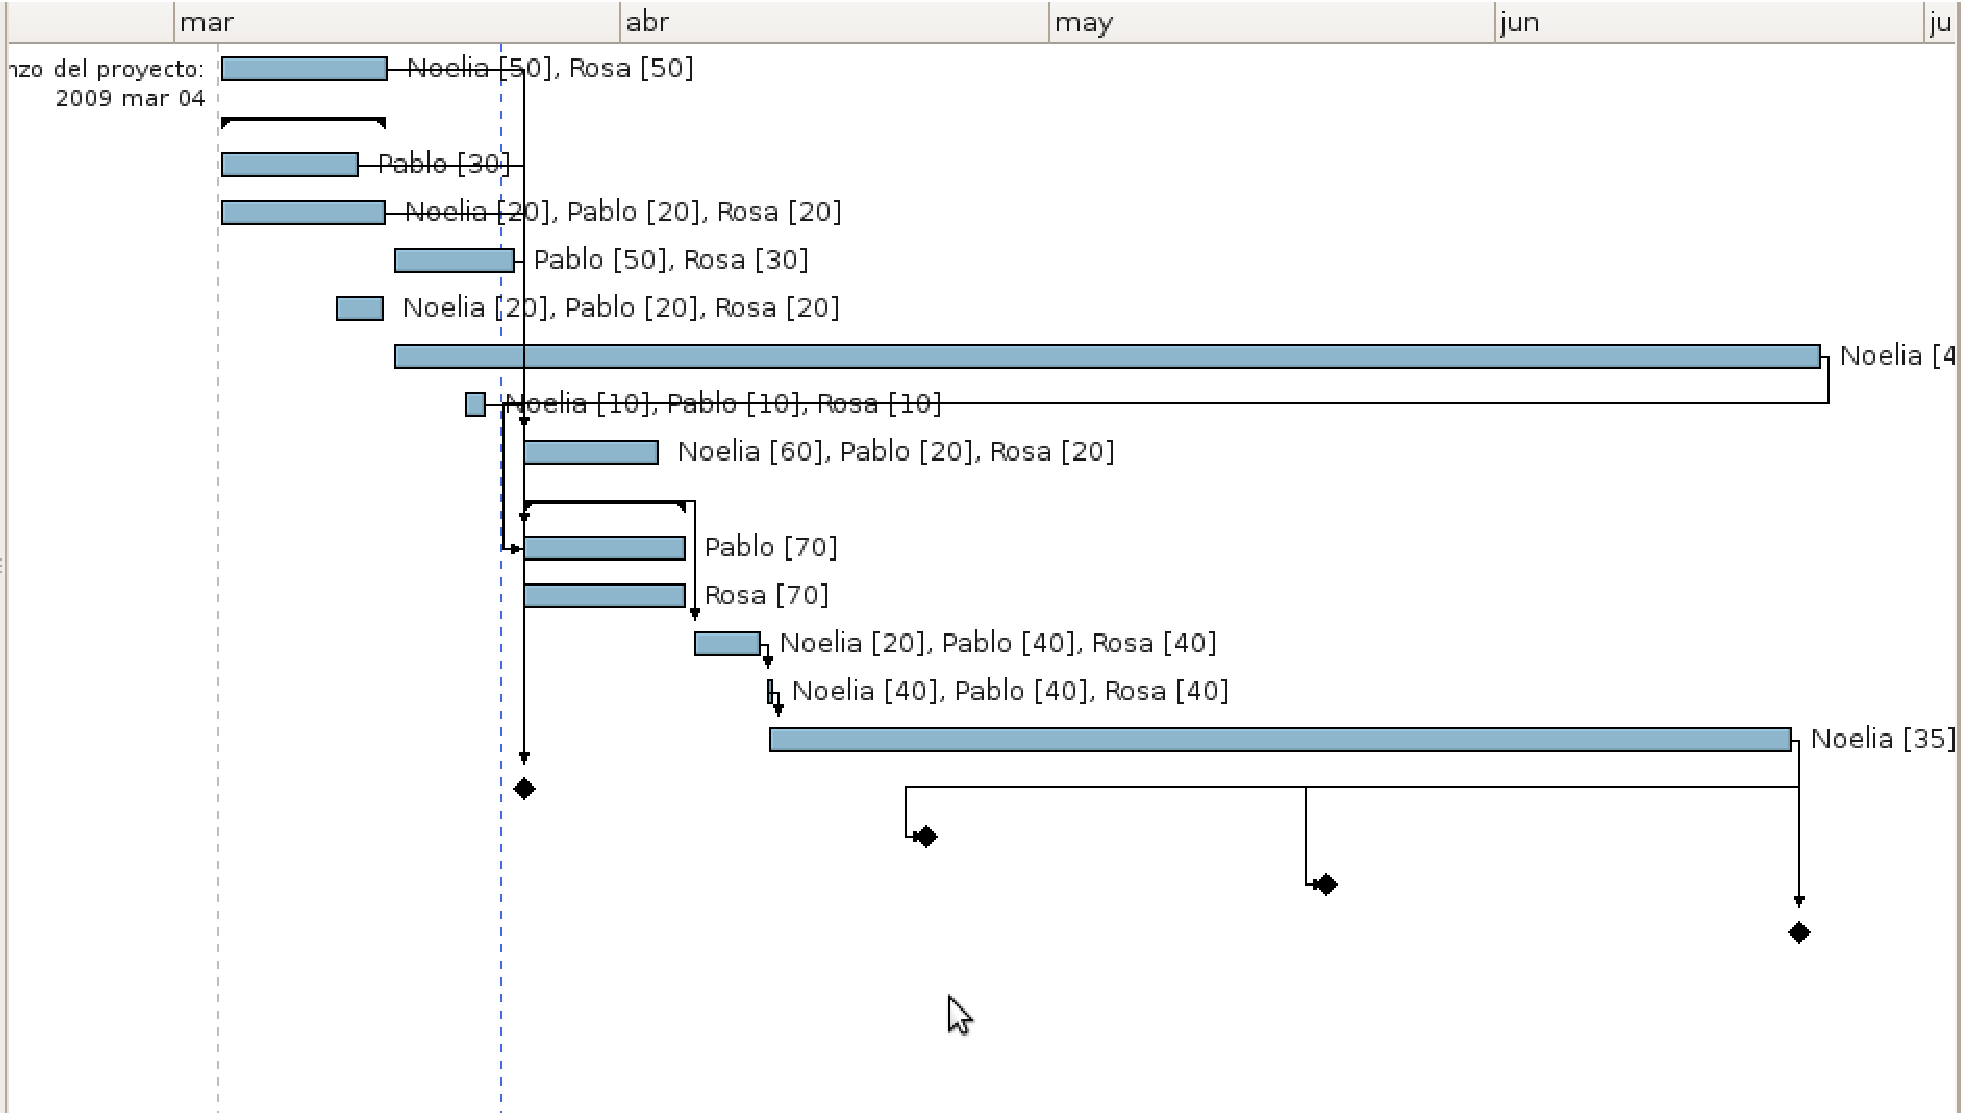
\includegraphics[scale=0.27]{./Imagenes/gannt.pdf}
   \end{figure}
  \end{frame}

  \begin{frame}{Coste}
    \transdissolve
    \begin{block}{Gracias a Planner...}
      \noindent Asignando a cada hora de trabajo 6 Euros, según
      Planner, el proyecto tiene un coste inicial de \textbf{8363,17
        EUROS}... lo cual es una cifra considerable.
    \end{block}
  \end{frame}
  

 \section{Partes del juego}
 
  \subsection{Sistemas o motores}
  
  \begin{frame}{Dos motores necesarios...}
   \transdissolve
   
   \begin{description}
    \item[Movimiento: ] Vista a priori cenital, con el movimiento del
	       personaje principal por el mundo, de un punto a otro del
	       mapa, obteniendo objetos y desarrollando la historia.
    \item[Combate: ] El sistema de combate será totalmente
	       independiente; otro tipo de gráficos y de reglas de
	       movimiento.
   \end{description}
   
  \end{frame}
  
  \subsection{Historia y personajes}
  
  \begin{frame}{Nombres}
   \transdissolve
   
   El nombre definitivo del proyecto es \textsc{NoCKt
   Metal}, el grupo protagonista \textsc{The Ampli Breakers} y los
   4 personajes:
   \begin{itemize}
    \item \textbf{Manololapunki} $\longrightarrow$ Cantante
    \item \textbf{Dentacos Joe} $\longrightarrow$ Guitarra
    \item \textbf{Baldos} $\longrightarrow$ Batería
    \item \textbf{Graimito el Bajo} $\longrightarrow$ Bajista
   \end{itemize}
   
  \end{frame}
  
  \subsection{Diseño gráfico}
  
  \begin{frame}{Primeros sprites}
   \transdissolve
   
   \begin{block}{¿Hay gráficos hechos?}
   Se han empezado a desarrollar los gráficos incluyendo los menús (tanto el básico como el de combate) así como el diseño de los personajes principales.
   \end{block}
   
   \pause
   
   \begin{figure}[t]
    \centering
    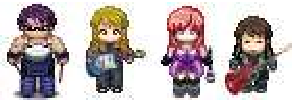
\includegraphics[scale=1]{./Imagenes/grupo.pdf}    
   \end{figure}
  \end{frame}
  
  
  
  \begin{frame}{Sprites de movimiento completos}
   \transdissolve
   
   \begin{figure}[t]
    \centering
    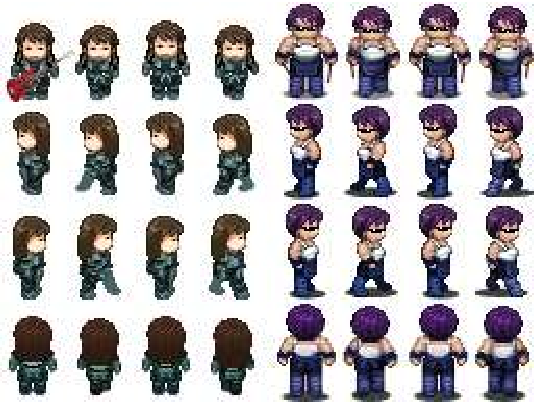
\includegraphics[scale=0.9]{./Imagenes/bajo_bateria.pdf}    
   \end{figure}
  \end{frame}
  
  
  \begin{frame}{Sprites de movimiento completos}
   \transdissolve
   
   \begin{figure}[t]
    \centering
    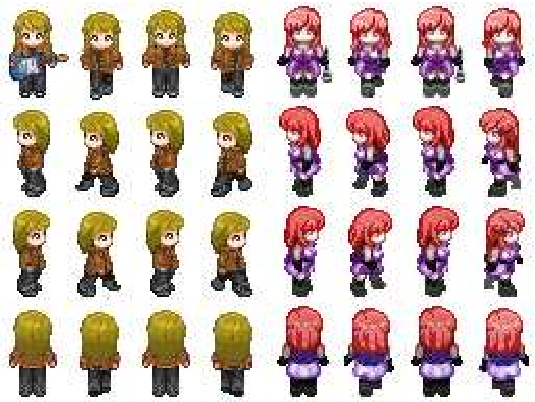
\includegraphics[scale=0.9]{./Imagenes/guitarra_cantante.pdf}    
   \end{figure}
  \end{frame}
  
  \section{Para finalizar}
  
  \subsection{Enlaces de interés}
  
  \begin{frame}{Enlaces de interés}
   \transdissolve
   
   \begin{itemize}
   \item Enlace a la forja del proyecto:
   
  \url{https://forja.rediris.es/projects/nocktmetal/}
  
  \item Convención de estilo de programación (Proyecto \textsc{ScummVM}):
  
  \url{http://wiki.scummvm.org/index.php/Code_Formatting_Conventions}
   \end{itemize}
  \end{frame}
  
  
  \subsection{Para terminar}
  
  
  \begin{frame}{Para terminar...}
   \transdissolve
   
   \begin{center}
   \Large Hasta la próxima presentación\\
   
   \Huge Powered by \LaTeX\\[3cm]
   \end{center}
   
   \normalsize
   
   PD: Abraham, ¿nos echas una manita con el audio? :P
   
  \end{frame}
  
\end{document}
